In Fig.~\ref{fig:roc_and_pr_curves_MIMIC}, and Fig.~\ref{fig:roc_and_pr_curves_eICU}, we provide the full ROC and PR curves for all possible objectives for training logistic regression on MIMIC and eICU.
We see that our proposed method delivers noticeable gains especially in the precision-recall curve, which we argue is more suitable to early warning systems.


\begin{figure*}[!h]
\centering
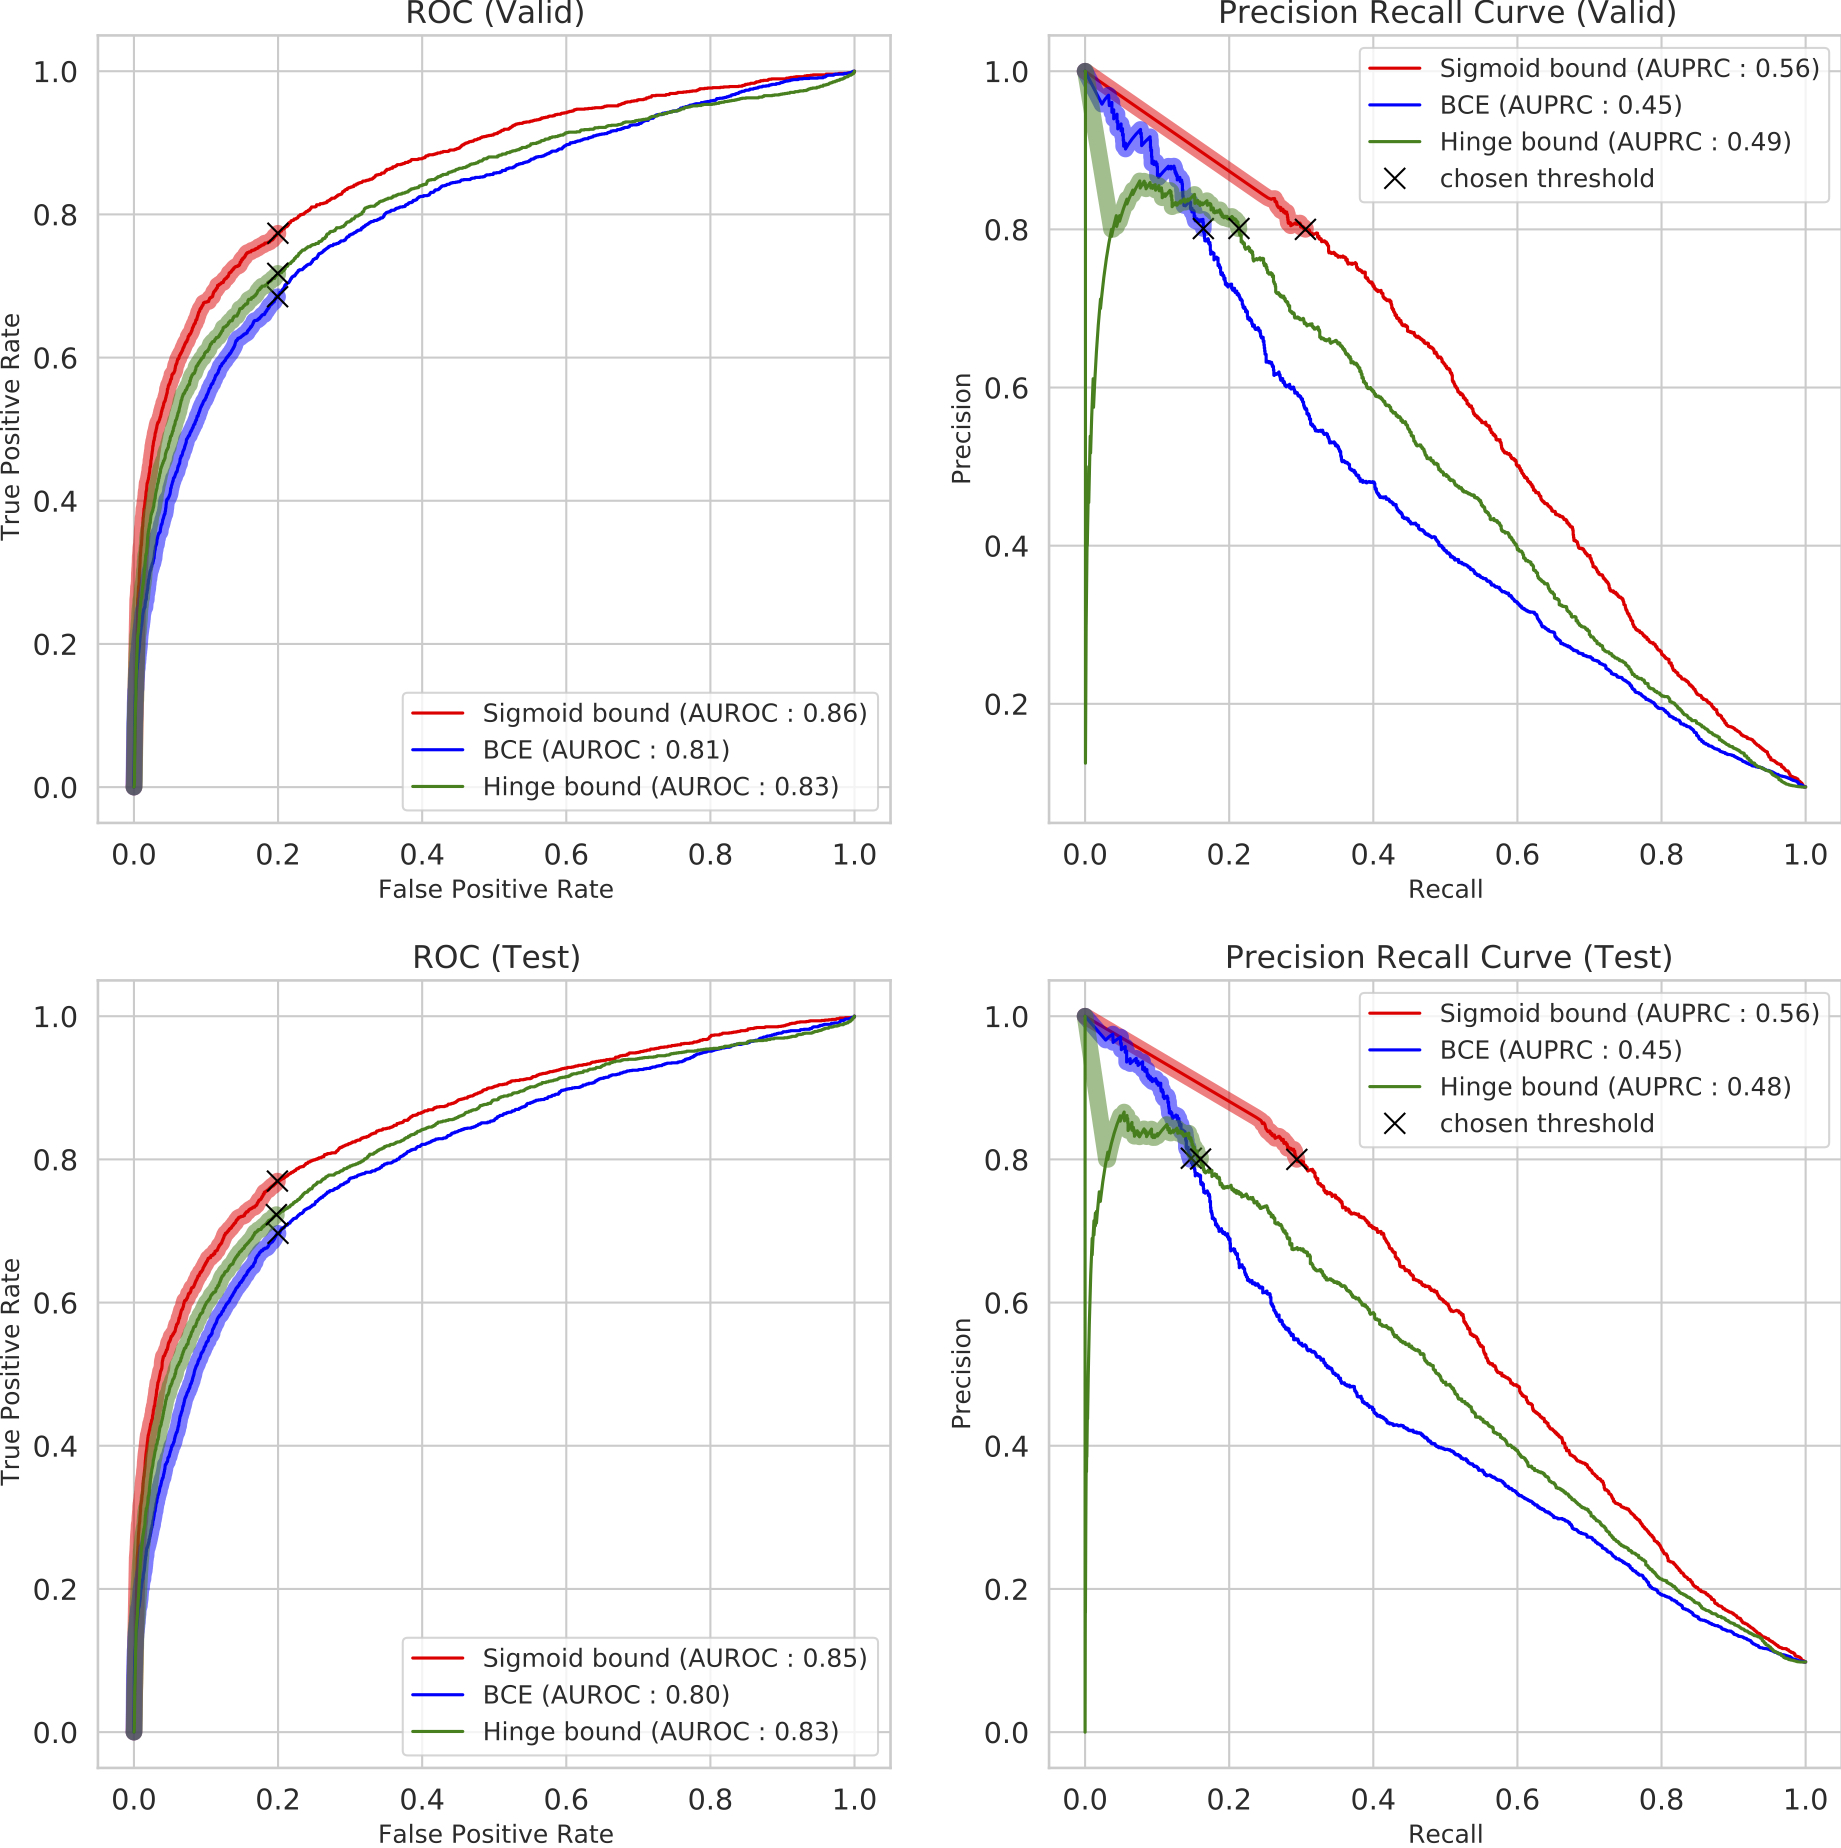
\includegraphics[width=0.8\textwidth]{content/chapters/false_alarm_control/figures/roc_prc_all_methods_mimic.jpg}
\caption[ROC curves for models trained on MIMIC using different optimization objectives]{
\textbf{Receiver operating curve (ROC, left column) and precision-recall curve (PR, right column) for logistic regression models trained using different optimization objectives on the MIMIC dataset} (top row: validation set; bottom row: test set).
Each curve shows tradeoffs in performance metrics possible while varying the decision threshold $b$ of a single method.
\emph{Left column:} Receiver operating curve (ROC), comparing true positive rate (TPR, y-axis) to false positive rate (FPR, x-axis).
\emph{Right column:} Precision-recall curve, comparing precision (also known as positive predictive value (PPV), y-axis) to recall (also known as TPR, x-axis).
Our sigmoid bound and \citet{ebanScalableLearningNonDecomposable2017}'s hinge bound were trained to maximize recall subject to a constraint on precision: above 0.9 on training set; above 0.8 on validation set. \emph{Darker line segments} indicate thresholds satisfying the desired precision above 0.8 on validation set.
\emph{The black ``X'' marker} indicates the selected operating point for each method (chosen to maximize our optimization objective on the validation set).}
%endcaption	
\label{fig:roc_and_pr_curves_MIMIC}
\end{figure*}

\begin{figure*}[!h]
\centering
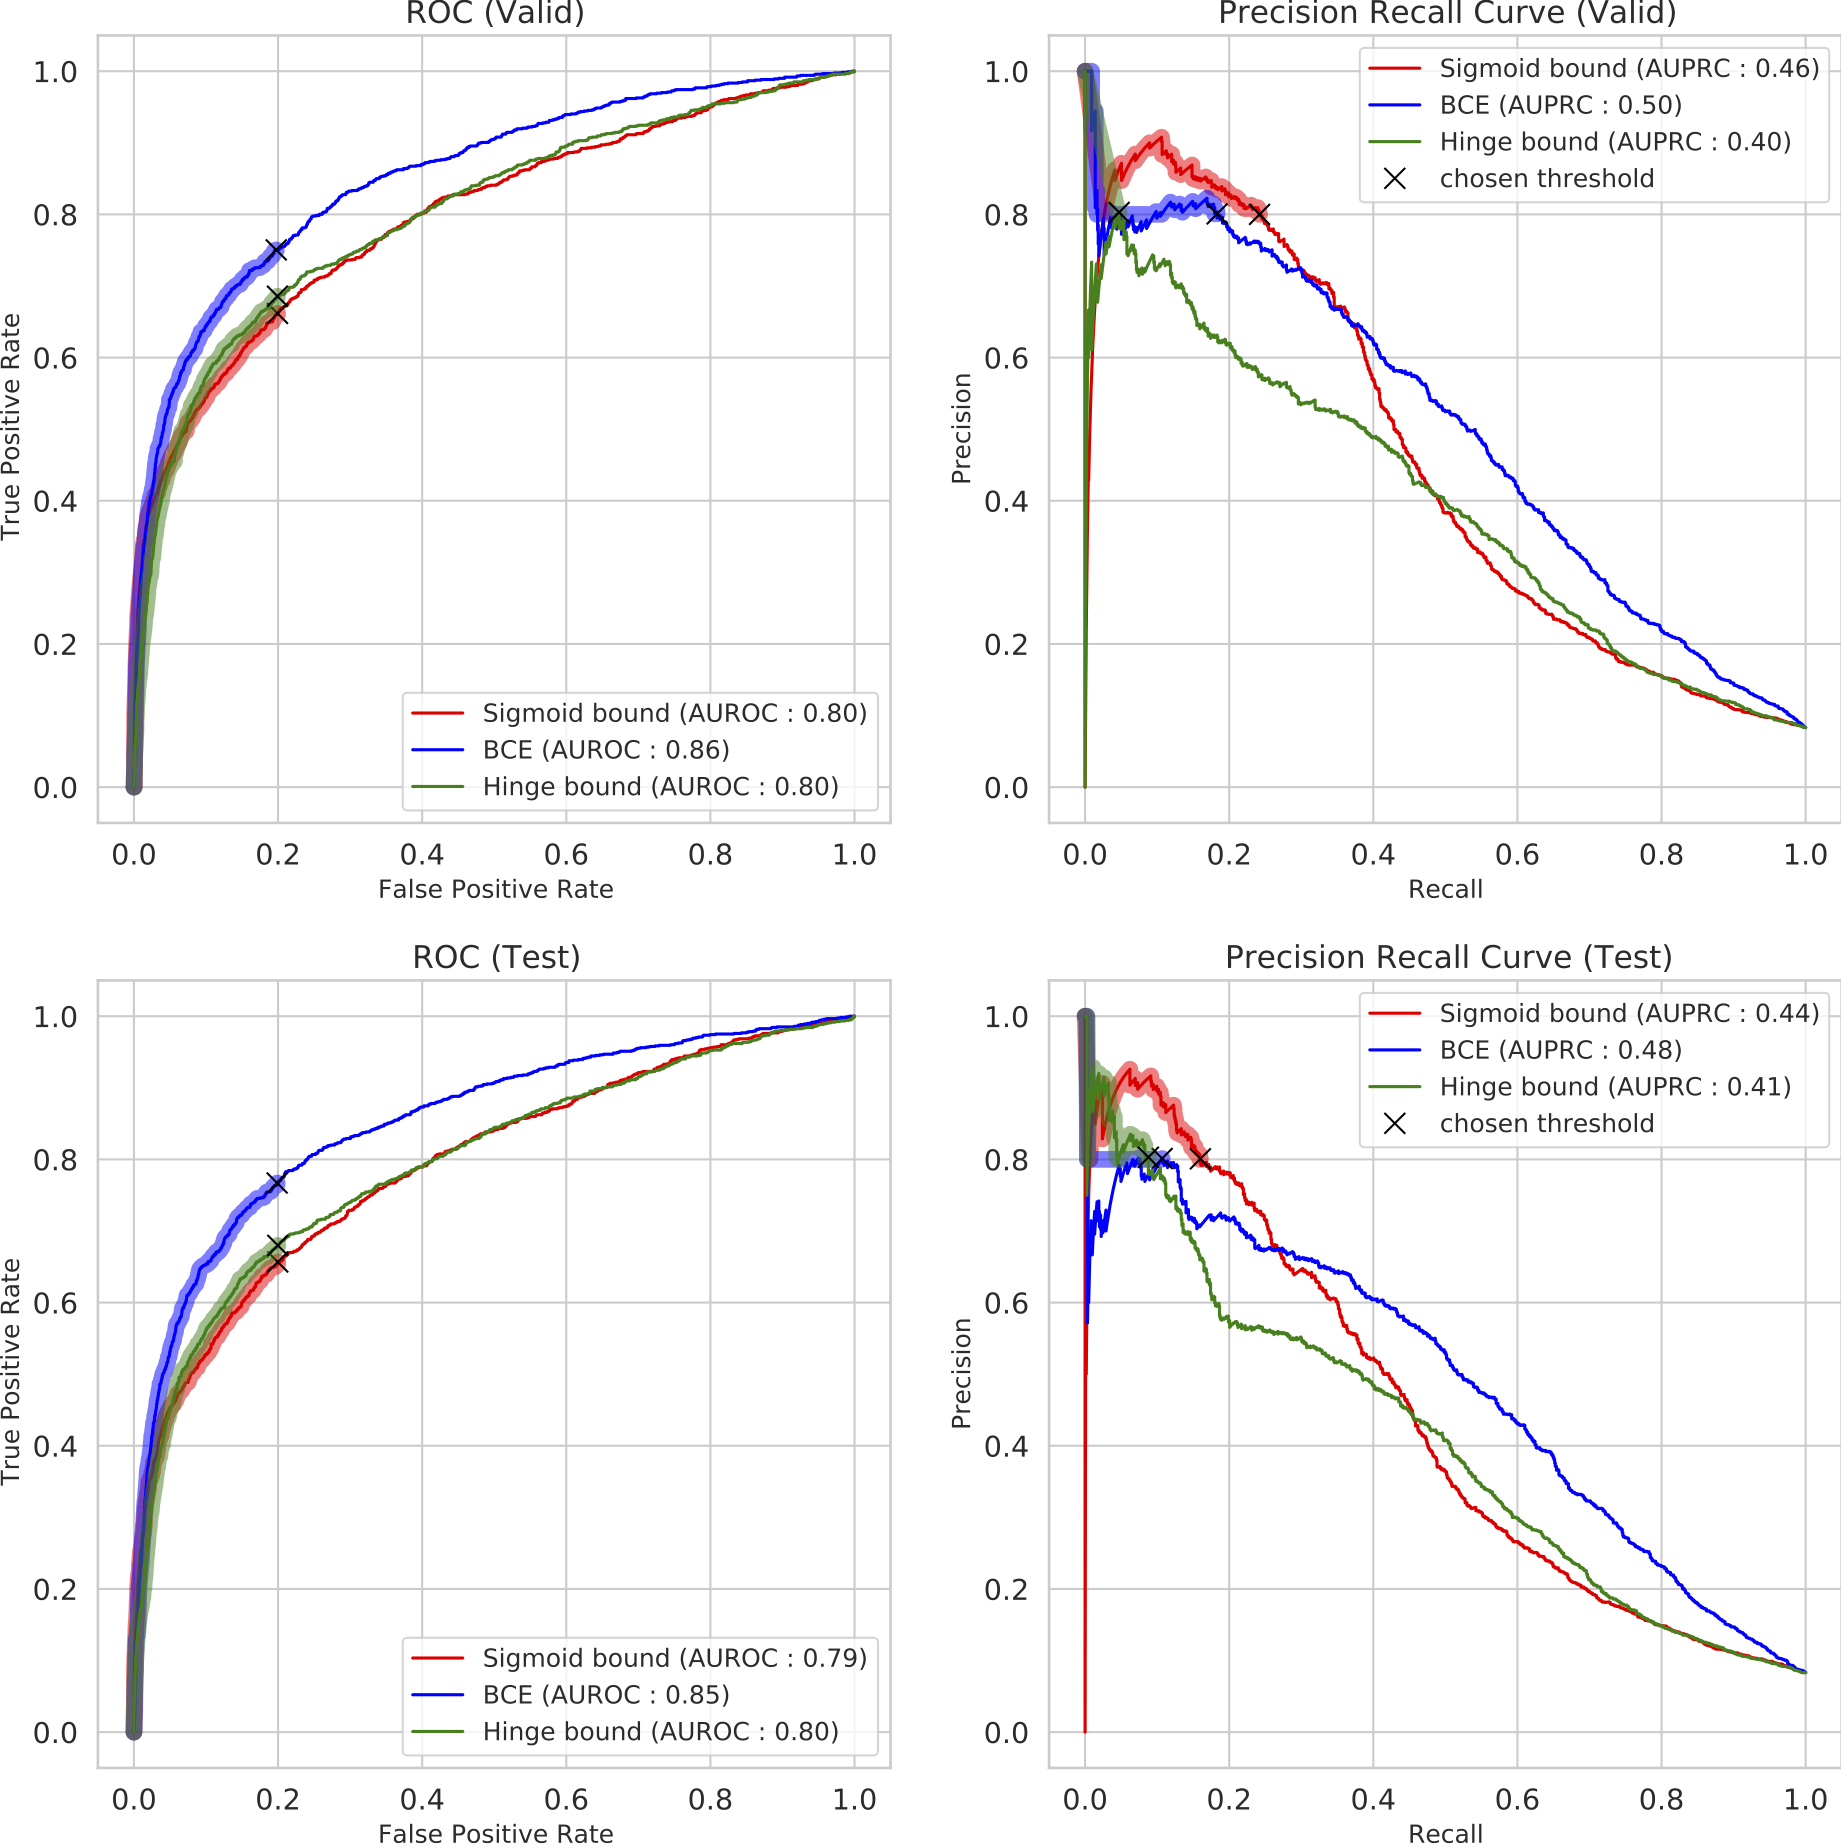
\includegraphics[width=0.8\textwidth]{content/chapters/false_alarm_control/figures/roc_prc_all_methods_eicu.jpg}
\caption[ROC curves for models trained on eICU using different optimization objectives]{
\textbf{Receiver operating curve (ROC, left column) and precision-recall curve (PR, right column) for logistic regression models trained using different optimization objectives on the eICU dataset} (top row: validation set; bottom row: test set).
Each curve shows tradeoffs in performance metrics possible while varying the decision threshold $b$ of a single method.
\emph{Left column:} Receiver operating curve (ROC), comparing true positive rate (TPR, y-axis) to false positive rate (FPR, x-axis).
\emph{Right column:} Precision-recall curve, comparing precision (also known as positive predictive value (PPV), y-axis) to recall (also known as TPR, x-axis).
Our sigmoid bound and \citet{ebanScalableLearningNonDecomposable2017}'s hinge bound were trained to maximize recall subject to a constraint on precision: above 0.9 on training set; above 0.8 on validation set. \emph{Darker line segments} indicate thresholds satisfying the desired precision above 0.8 on validation set.
\emph{The black ``X'' marker} indicates the selected operating point for each method (chosen to maximize our optimization objective on the validation set).}
%endcaption	
\label{fig:roc_and_pr_curves_eICU}
\end{figure*}